\section{Projektüberblick}

\begin{frame}{Tools}
	\begin{itemize}
		\item Java, Eclipse, Android ADT
		\item Git
		\item UMLet, ArgoUML
		\item Emma, EclEmma
	\end{itemize}
\end{frame}

\begin{frame}{Statistiken}
	\begin{itemize}
		\item 170 Klassen (13000 Lines of Code)
		\item 250 Testfälle (4600 Lines of Code)
		\item 600 Zeilen Integrationstests in Python
		\item 96\% Testabdeckung im Model, 78\% gesamt
	\end{itemize}
\end{frame}

\begin{frame}{Danke für's Zuhören}
	\begin{center}
		\textcolor{blue}{\href{http://github.com/TeamCroggle}{http://github.com/TeamCroggle}}
		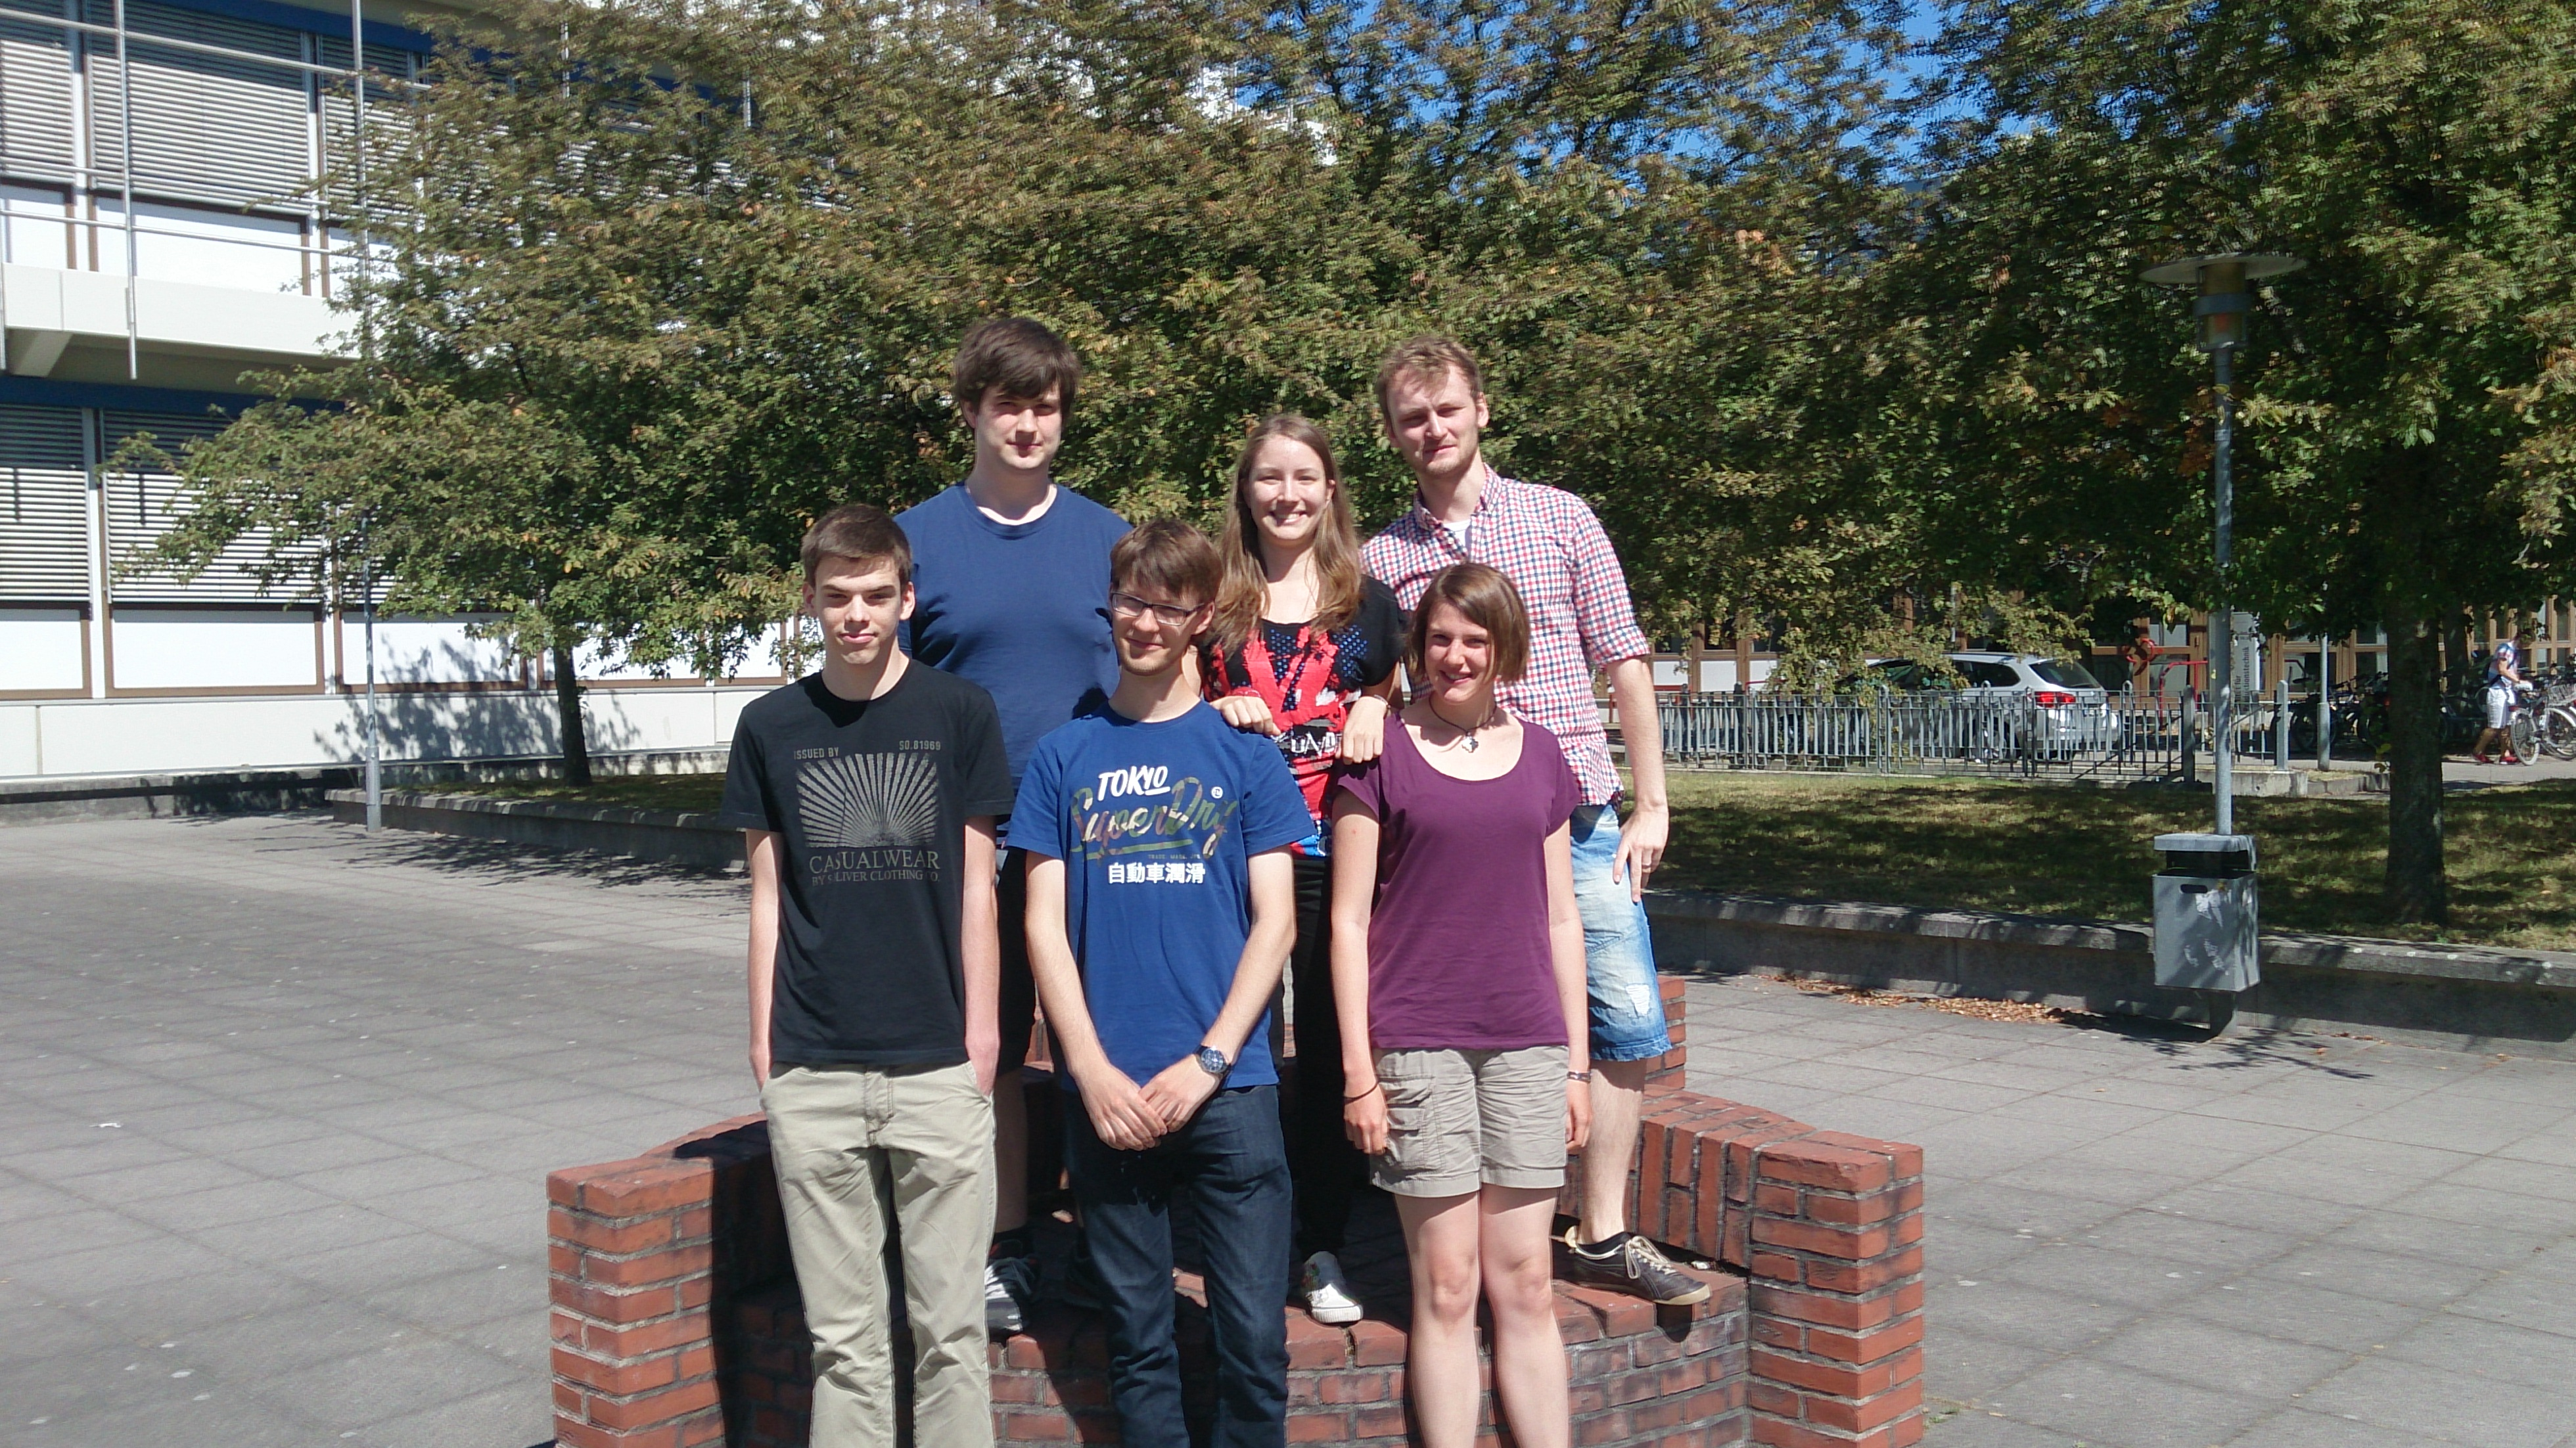
\includegraphics[width=10cm,type=jpg,ext=.jpg,read=.jpg]{media/2014-06-24 10.56.29}
	\end{center}
\end{frame}
